\chapter[Analiza problemu]{Analiza problemu}

\label{chapter:analiza_problemu}

% W tym rozdziale trzeba bardziej szczegółowo opisać jak chce Pan
% zrealizować cele sformułowane w rozdziale 2.
% Jakie będą konsekwencje i ewentualne wyzwania techniczne
% związane z przyjętą strategią. Jaka ogólnie ma być komunikacja
% z komputerem, tzn. czy to ma być tryb pytanie-odpowiedź, czy ciągłe
% przesyłanie danych. Czy być może jakiś tryb mieszany.
% Jaką chce Pan przyjąć formę przetwarzania danych i dlaczego. itd. itd.


\section{Plan urządzenia}

Założenia konstrukcyjne to przede wszystkim prostota budowy, modularność i skrócenie czasu realizacji. 
Płytka deweloperska wysyła określoną przez użytkownika liczbę przebiegów sygnału PWM (Pulse Width Modulation), 
następnie sygnał jest ten wzmacniany 
do poziomu aż \unit[80]{V} by uzyskać maksymalną wydajność i trafia na przetwornik piezoelektryczny który generuje falę ultradźwiękową.
Fala ta po odbiciu się od obiektu w polu wykrywania sonaru trafia z powrotem do urządzenia a konkretniej do mikrofonów MEMS umieszczonych na czole obudowy.
Sygnał z mikrofonów jest filtrowany by przepuścić tylko porządane przez nas częstotliwości bliskie czestotliwości nadajnika, 
oraz wzmacniany w celu lepszej interpretacji przez dalsze układy.

Po przefiltrowaniu, sygnał jest progowany. Mikrokontroler za pomocą przetwornika DAC ustala poziom napięcia, 
który wyznaczy granicę pomiędzy wysokim a niskim stanem logicznym. To rozróznienie jest nam potrzebne do pobudzenia cyfrowego wejścia licznika, 
zmienność tej wartości pozwala nam również na reagowanie tylko na sygnał o odpowiedniej amplitudzie by móc z powrotem obniżyć próg 
do miejsca przecięcia się sinusoidy z napięciem odniesienia, gdzie dokładność pomiaru jest największa.
Mikroprocesor dzięki wspomnianym wcześniej licznikom odmierza czas między zboczami rosnącymi zprogowanego już sygnału.
Wszystkie pomiary czasów przecieć z trzech odbiorników są wysyłane we wspólnej ramce danych do komputera gdzie za pomocą 
różnic w tych czasach wyznaczony zostanie dystans obiektu oraz jego odchylenie względem sonaru. Rys \ref{fig:uml}
\begin{figure}[ht!]
    \centering
    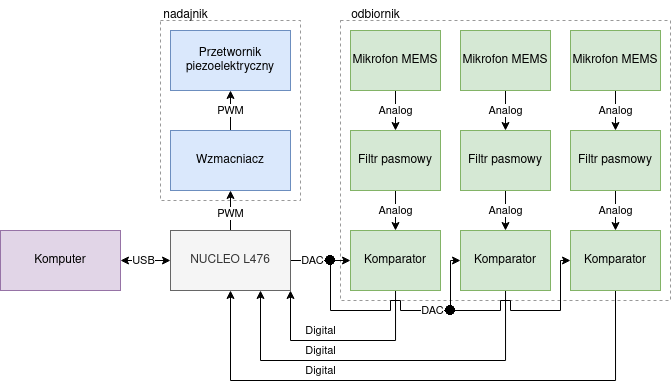
\includegraphics[width = 0.8\textwidth]{sonar_uml.png}
    \caption{Schemat blokowy urządzenia}
    \label{fig:uml}
\end{figure}



\section{Rozmieszczenie elementów nadawczych i odbiorczych}
Rozmieszczenie odbiorników jest kluczowym elementem pomiaru, to dzięki znajomości odległości mikrofonów i różnic w czasach 
dotarcia sygnału jesteśmy w stanie określić kąt pod którym fala dźwiękowa trafia do urządzenia. 
Do uzyskania pełnego zakresu w trzech osiach, wymagane są co najmniej trzy odbiorniki:
\begin{itemize}
    \item Mikrofon 0 -- mikrofon odniesienia, znajduje się on w centralnym punkcie, to według niego wyznacza będzie odległość od obiektu.
    \item Mikrofon X -- na podstawie pomiaru z tego mikrofonu wyznacza się kąt odchylenia w osi X 
    \item Mikrofon Y -- na podstawie pomiaru z tego mikrofonu wyznacza się kąt odchylenia w osi Y
\end{itemize}

\begin{figure}[ht!]
    \centering
    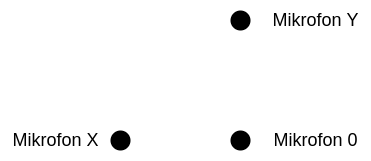
\includegraphics[width = 0.5\textwidth]{rozmieszczenie_mic.drawio.png}
    \caption{Rozmieszczenie mikrofonów}
    \label{fig:rozmieszczenie_mic}
\end{figure}

\section{Generowanie i odbieranie sygnału ultradźwiękowego}

\section{Komunikacja}
Komunikacja komputera typu PC z płytką deweloperską Nucleo na której bazowany jest projekt odbędzie się przy pomocy portu szeregowego. 
Każdy nowoczesny komputer posiada złącze USB, które miało niezwykły wpływ na standaryzacje interfejsów w urządzeniach użytkowych, 
większość płytek deweloperskich również posiada wbudowane gniazdo USB z portem szeregowym, dlatego też wybór tego rodzaju kompunikacji wydaję się wręcz oczywistą decyzją.
Tym samym złączem wgrywany jest również program do pamięci mikrokontrolera co jeszcze bardziej upraszcza stanowisko testowe.
Dane będą wysyłane w postaci tekstu w formie ,,pytanie-odpowiedź", zagwarantuje to większą elastyczność i możliwość zmiany parametrów urządzenia bez konieczności zmiany programu. 
W celu uruchomienia sekwencji wykrywania obiektu operator powinień wysłać komendę przykładowo o nazwie "START". 
Komenda taka posiadać będzie swoje ID w formie pojedynczej cyfry, pozwoli to zmniejszyć ilość znaków zamieszczanych w ramce danych. 
Komunikacja tekstowa przede wszystkim pozwala na weryfikacje danych przez standardowy terminal tekstowy. 
Ramka danych rozpocznie się znakiem ,,X", pomoże to programowi odfiltrować tylko dane przeznaczone dla niego. ,,X" został wybrany ze wględu na to, 
że znak ten na pewno nie będzie występował w treści wiadomości w żadnej postaci.
Wiadomość startu wraz z opcjonalnymi parametrami takimi jak ilość impulsów do wyemitowania czy próg czułości wykrywania sygnału wysłane są bajt po bajcie do urządzenia. 
Sonar rozpoznając znak początku ramki przechodzi dalej do odczytywania ID komendy oraz jej parametrów, po odebraniu całej wiadomości program zaczyna sekwencję pomiaru.
Następnie urządzenie wysyła do użytkownika odpowiedź, standardowo zaczyna znakiem rozpoznawczym a następnie zwraca numer ID komendy na którą ta wiadomość jest odpowiedzią,
status wykonania zadania, w formie kodów błędów, liczba wykrytych przecieć zer, czas kontrolny\todo{sprawdzić czy na pewno}, oraz wartości liczników z każdego ze składowych pomiaru.
Dane będą przetwarzane przez operacje na obiektach typu {\tt string}. Pozwoli to na wycięcie odpowiednich wartości ze scalonej ramki wysłanej jako jeden długi ciąg znaków.


% Lorem ipsum: \todo{jak dane są wyciagane z ramki, ogólny opis, port szeregowy, czemu tekstowo?}
% wybrano komunikacje tekstwoa co pozwalaa na zweryfikowanie danych poprzez zwykly teminal tekstowy nie powoduje obnizenia ofektywnosci kominikacji urzadzenia z komputerem 
% przyjeto komunikacja zapytanie odpowiedz, ze wzgledu na wieksza elastycznosc i mozliwosc zmiany ustawien sonaru 
% funkcje


